% !Mode:: "TeX:UTF-8" (encoding info for WinEdt)
\section{Elexis-Befunde}
Einbindung textorientierter datierter Befundserien (z.B. Gewicht, BZ, Quick etc.). Dieses Plugin ist Teil der Standard-Distribution.
\subsection{Konfiguration}

Wenn das Plugin installiert ist, finden Sie im Menu Datei-Einstellungen eine Rubrik \textit{Befunde}. Diese wird anfangs leer sein (Abb. \ref{fig:befundesettings}):
\begin{figure}[htp]
    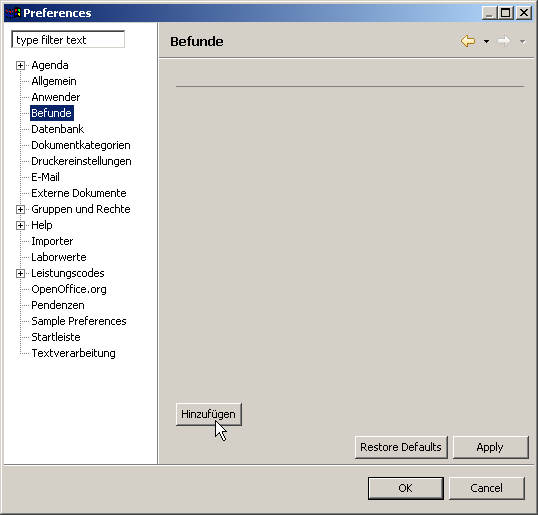
\includegraphics[width=4in]{images/befunde1.png}
    % befunde1.png: 538x515 pixel, 96dpi, 14.23x13.62 cm, bb=0 0 403 386
    \caption{Befunde-Einstellungen}\label{fig:befundesettings}
\end{figure}


Um einen neuen Befundparameter hinzuzufügen, klicken Sie auf  \textit{Hinzufügen}. Sie werden nach dem Namen dieses Parameters gefragt, wir wählen  Röntgen. Danach erscheint eine Karteikarte mit diesem Parameter, die wir jetzt noch mit den einzutragenden Datenspalten versehen müssen (Abb: \ref{fig:befunde2}).
\begin{figure}[htp]
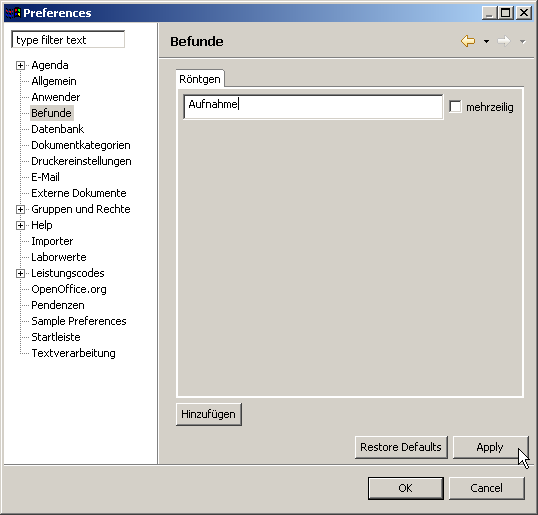
\includegraphics[width=3in]{images/befunde2.png}
% befunde2.png: 538x515 pixel, 96dpi, 14.23x13.62 cm, bb=0 0 403 386
    \caption{Neuer Parameter}\label{fig:befunde2}
\end{figure}
Klicken Sie nach jeder Zeile auf  \textit{Apply}  bzw.  \textit{Anwenden}:
\begin{figure}[htp]
    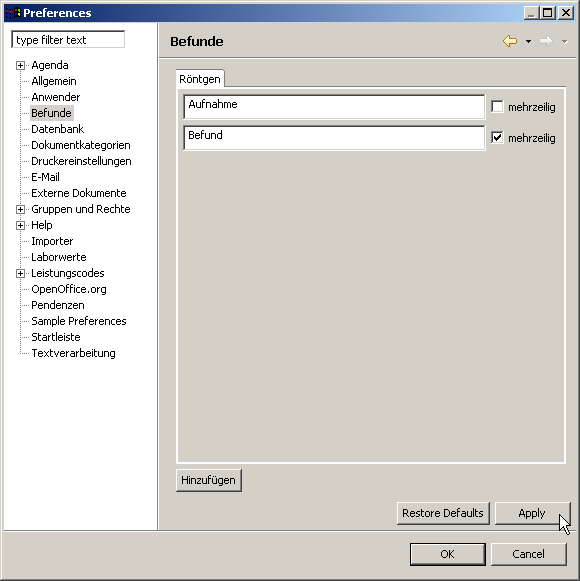
\includegraphics[width=3in]{images/befunde3.png}
    % befunde3.png: 580x581 pixel, 96dpi, 15.34x15.37 cm, bb=0 0 435 436
        \caption{Neuer Parameter 2}\label{fig:befunde3}
\end{figure}

Wenn ein Feld mehrzeilig sein soll, klicken Sie die entsprechende Checkbox an. Eine Variante mit mehr als zwei Spalten sehen Sie in Abb. \ref{fig:befunde4}.:
\begin{figure}[htp]
    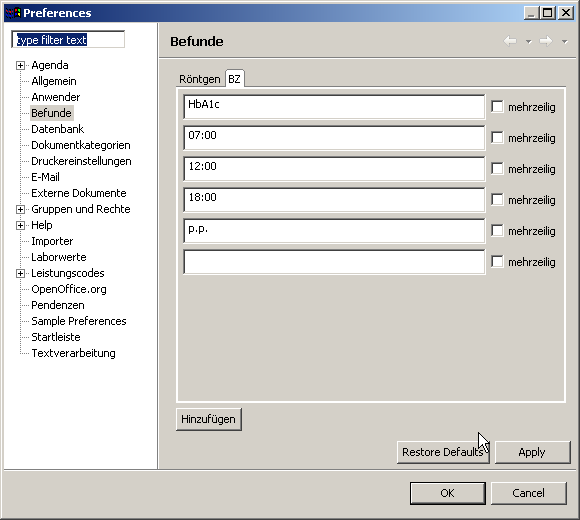
\includegraphics[width=4in]{images/befunde7.png}
    % befunde7.png: 580x520 pixel, 96dpi, 15.34x13.76 cm, bb=0 0 435 390
    \caption{Mehrspaltiger Parameter}\label{fig:befunde4}
\end{figure}

\pagebreak

\subsection{Anwendung}

Öffnen Sie die  Befunde-View.
\begin{flushleft}
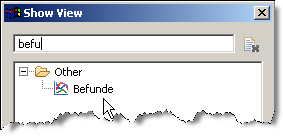
\includegraphics[width=3in]{images/befunde4.png}
% befunde4.png: 276x394 pixel, 96dpi, 7.30x10.42 cm, bb=0 0 207 295
\end{flushleft}

Sie sehen dann die konfigurierten Messparameter:
\begin{flushleft}
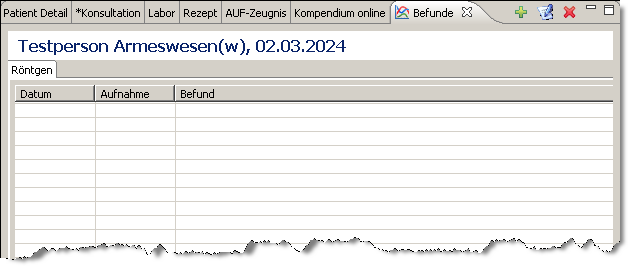
\includegraphics[width=4in]{images/befunde5.png}
% befunde5.png: 621x636 pixel, 96dpi, 16.43x16.83 cm, bb=0 0 466 477
\end{flushleft}
Um eine neue Messung einzugeben, klicken Sie auf das grüne Pluszeichen rechts oben.
\begin{flushleft}
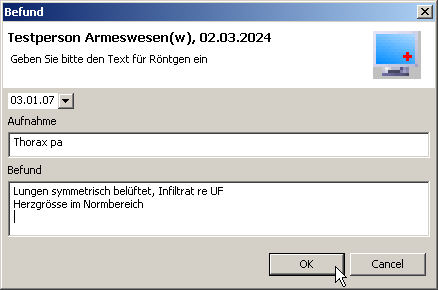
\includegraphics[width=3in]{images/befunde6.png}
% befunde6.png: 438x290 pixel, 96dpi, 11.59x7.67 cm, bb=0 0 328 217
\end{flushleft}
Sie sehen jetzt Ihre bei der Konfiguration angegebenen Messzeilen, ein- oder mehrzeilig. Mit Klick auf OK wird der neue Eintrag übernommen. Mit Doppelklick können Sie ihn wieder öffnen.
